\chapter{Fig, table and Code}

\section{Code}

\subsection{Inline code}
Use \lstinline|\lstinline$<code>$| to print the code snippets. The exclamation marks delimit
the code and can be replaced by any character not in the code;
\lstinline|var i:integer;| gives the same result.

\section{Figure}

\begin{figure}[!htb]
  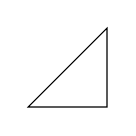
\begin{tikzpicture}
    \draw (0,0) -- (1, 0) -- (1, 1) -- cycle;
  \end{tikzpicture}
  \caption{An example tikz picture}
  \label{fig:tikz example}
\end{figure}

You can use \lstinline|\cref{}| to automatically setup the cross reference name; instead, you can always use \lstinline|\ref{}| to customize the appearence of the cross reference.

An example image is shown in \cref{fig:tikz example} or Figure (\ref{fig:tikz example}).
